\section{Study case: experiments and evaluation}
To evaluate our system we need some initial data to define the \textit{relevances} (see section \ref{section:context-awareness}) and some (real or simulated) users to test with.

\subsection{Relevances} \label{section:relevances-survey}
To define each $r_{c,x}$ for each node $c$ and context factor $x$, it was decided to gather real data provided by real people through a survey and then average them. The survey consisted of the question "Answer how much a 'context factor' influences your decision to go to a place/event of the specified type (these types are not exclusive)". Then, for each of the ontology classes specified on section \ref{section:context_factors} people had to answer a real value between $0$ and $10$, where:
\begin{itemize}
    \item $0$ means that if the context factor is met, you would not go to the place / event.
    \item 5 means you don't care if the context is met or not.
    \item 10 means that if the context is met, you would go to the place / event.
\end{itemize}

Then the following formula is applied to each feature or column, hence average them and transforming them to be on range $[0,2]$:
$$AVG(column)/5$$

The form had a total of 34 answers. Something worth to mention was that the answers were concentrated between the options $0$, $5$ and $10$, maybe because it is easier to think something between the thoughts "I would not", "I don't care" and "I would", than to think something that is in the middle of two of those thoughts.

\subsection{Users data}
As explained before (see section \ref{section:preferences-propagation}), a user of the system have to give initial preferences to some ontology classes. It was decided to make a form where people could answer their preferences of the higher level ontology classes mentioned before (see section \ref{section:context_factors}). The form had a total of 63 answers. The genre, country, profession, age and (optional) social networks were also asked to have more information for further work. The answer should be integers on range $[1, 10]$. Again, answers were more concentrated on the middle and highest options, but there were few low answers.

\subsubsection{Simulated scenarios}
To evaluate the system, it was decided to test it with simulated scenarios (simulated contexts and simulated users). A set of centroids of a set of clusters were chosen as the set of simulated users. The \textit{K-Means} algorithm was used to get the clusters and the \textit{Elbow Method} (see figure \ref{fig:elbow}) was used to choose $4$ as the number of clusters.
\begin{figure}[h]
    \centering
    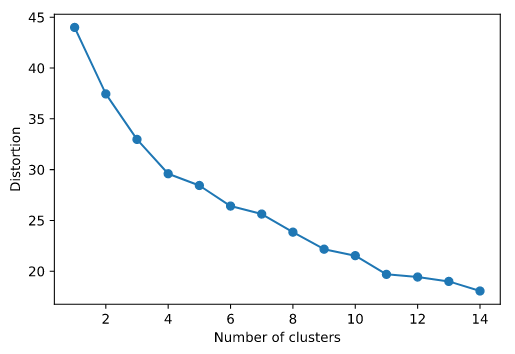
\includegraphics[scale=0.45]{elbow.png}
    \caption{Distortions of the different number of clusters}
    \label{fig:elbow}
\end{figure}

The centroids of the found clusters can be seen on table \ref{table:centroids}. On figure \ref{fig:tourist_hist} we can see how are initial preferences distributed for each tourist.
\begin{table}[h!]
\centering
\begin{tabular}{ |c|c|c|c|c| } 
    \hline
    Class & $T_1$ & $T_2$ & $T_3$ & $T_4$ \\
    \hline
    \hline

    Museum & 0.7235 & 0.6476 & 0.78 & 0.9421 \\ 
    \hline
    Interpretation Center & 0.6824 & 0.6476 & 0.52 & 0.8737 \\
    \hline
    Library & 0.5588 & 0.46667 & 0.72 & 0.7684 \\
    \hline
    Park and Garden & 0.865 & 0.8714 & 0.7 & 0.9316 \\
    \hline
    Archaeological Site & 0.6882 & 0.8619 & 0.82 & 0.826 \\
    \hline
    Religious Site & 0.45882 & 0.7 & 0.36 & 0.7316 \\
    \hline
    Remarkable Building & 0.6529 & 0.8524 & 0.4 & 0.7895 \\
    \hline
    City Heritage & 0.7412 & 0.919 & 0.58 & 0.8632 \\
    \hline
    Defence Site & 0.5412 & 0.8529 & 0.68 & 0.7421 \\
    \hline
    Remembrance Site & 0.4941 & 0.781 & 0.8 & 0.7211 \\
    \hline
    Technical Heritage & 0.4059 & 0.7905 & 0.56 & 0.5842 \\
    \hline
    Food Establishment & 0.9059 & 0.8905 & 0.7 & 0.6632 \\
    \hline
    Natural Heritage & 0.9059 & 0.9143 & 0.76 & 0.9211 \\
    \hline
    Sports & 0.9353 & 0.8429 & 0.22 & 0.6316 \\
    \hline
    Leisure Place & 0.9353 & 0.8429 & 0.22 & 0.6316 \\
    \hline
    Store & 0.7647 & 0.8286 & 0.28 & 0.5684 \\
    
    \hline
\end{tabular}
\caption{Centroids to be used as simulated users.}
\label{table:centroids}
\end{table}

\begin{figure}[h]
    \centering
    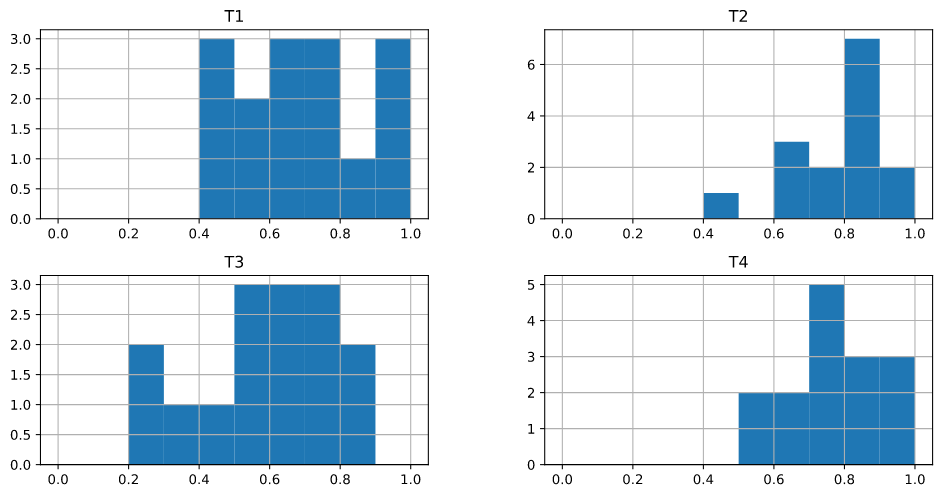
\includegraphics[scale=0.25]{tourist_histogram.png}
    \caption{Distributions of initial preferences of $T_1$, $T_2$, $T_3$ and $T_4$}
    \label{fig:tourist_hist} 
\end{figure}

\subsection{Metrics} \label{section:metrics}
For each centroid of the clusters mentioned previously, we simulate two visits to Niza, Lyon and Paris for each possible context using each possible value for each context factor. The system returns a set of not more than $5$ recommended places inside a radius of $8$ kilometers for each visit, this set is going to be called the \textit{recommendation}. Let $R$ be a recommendation for a specific user on a specific location and a specific context, we define the following recommendation metrics:
\begin{equation}
    pref_{R} = \frac{ \displaystyle \sum_{p \in R}{pref_p} }{|\lbrace p \ | \ p \in R \rbrace|}
\end{equation}

\begin{equation}
    act_{R} = \frac{ \displaystyle \sum_{p \in R}{act_p} }{|\lbrace p \ | \ p \in R \rbrace|}
\end{equation}

\begin{equation}
    \eta_{R} = \frac{ \displaystyle \sum_{p \in R}{\eta_p} }{|\lbrace p \ | \ p \in R \rbrace|}
\end{equation}

\begin{equation}
    dist_{u, R} = \frac{ \displaystyle \sum_{p \in R}{dist_{u, p}} }{|\lbrace p \ | \ p \in R \rbrace|}
\end{equation}

To compute novelty \cite{kotkov2016survey} we use the metric mentioned on section \ref{section:serendipity}, which is adapted as follows:
\begin{equation} \label{eq:novelty}
    nov_{u, p} = \  \underaccent{q \in rec(u)}{min} \  ( dist( c_p, c_q ) )
\end{equation}
where $p$ is a recommended place, $u$ the user to which $p$ was recommended, $rec(u)$ is the set of already recommended places to $u$, $c_p$ is the ontology class to which $p$ belongs and $dist$ computes the distance in the ontology (using \textit{Breadth First Search}) of two ontology classes. Finally, the system returns the average of each recommendation metric.

Now we can define the novelty of a recommendation as follows:
\begin{equation}
    nov_{u, R} = \frac{ \displaystyle \sum_{p \in R}{nov_{u, p}} }{|\lbrace p \ | \ p \in R \rbrace|}
\end{equation}

\subsection{Experiments}
We use different coefficients for the score (see section \ref{section:score}), and since we said $maxdist$ is $8$ for these experiments, we are ignoring it as argument. 

\subsubsection{First configuration}
First we consider $k_1 = 13/36$ for preference, $k_2 = 13/36$ for activation, $k_3 = 1/4$ for aging and $k_4 = 1/36$ for distance from user, resulting on equation \ref{eq:score-1} and giving more priority to preference and activation and very little priority to distance from user. With these parameters we start simulating each user and their visits.
\begin{equation} \label{eq:score-1}
    \begin{split}
        score_p = \ &\frac{13}{36} \cdot pref_c + \frac{13}{36} \cdot act_c \\
                                        &+ \frac{1}{4} \cdot \eta_p - \frac{1}{36} \cdot \frac{dist_{u,p}}{8}
    \end{split}
\end{equation}

We are showing some sets of recommended items like table \ref{table:t1-1}, where each $p_i$ is a recommended place and $score_{p_i} \ge score_{p_j}$ for every $i < j$. Table \ref{table:t1-1} corresponds to $T_1$'s first visit to Niza, on a rainy workday in the morning, where $p_1$ is Train des Merveilles (from class \textit{TouristTrain}), $p_2$ is Cinéma de Plein Air (from class \textit{Cinema}), $p_3$ is Casino de Beaulieu (from class \textit{Casino}), $p_4$ is Cinéma de Beaulieu (from class \textit{Cinema}) and $p_5$ is Lyon-style petanque fields (from class \textit{BoulesPitch}). We can see that since each of the places' ontology classes are subclasses of \textit{LeisurePlace}, which $T_1$ loves, they have same preference and activation and since this is the first recommendation, all aging values are $1.0$. Therefore, the distance is the tiebreaker. Despite of a rainy morning, the system recommends a tourist train to $T_1$, just because it is a leisure place.
\begin{table}[h!]
    \centering
    \begin{tabular}{ |c|c|c|c|c|c| } 
        \hline
        Field   & $p_1$ & $p_2$ & $p_3$ & $p_4$ & $p_5$ \\
        \hline
        $pref_c$    &  0.9353 & 0.9353 & 0.9353 & 0.9353 & 0.9353 \\
        $act_c$     & 4.4 & 4.4 & 4.4 & 4.4 & 4.4 \\
        $\eta_p$    & 1.0 & 1.0 & 1.0 & 1.0 & 1.0 \\
        $dist_{u,p}$ & 1.53 & 3.99 & 5.52 & 5.53 & 5.58 \\
        $score_p$    & 2.1713 & 2.1628 & 2.15745 & 2.15742 & 2.1573 \\
        
        \hline
    \end{tabular}
    \caption{First visit of $T_1$ to Niza with first configuration}
    \label{table:t1-1}
\end{table}


At the second visit to Lyon (see table \ref{table:t1-3}), on a rainy workday in the morning, only $p_1$ is not a leisure place but an interpretation center, a kind of place $T_1$ does not like as much as leisure places. However, the activation of \textit{InterpretationCenter} is higher enough to make $score_{p_1}$ greater than $score_{p_2}$. Despite of $p_1$ being very far away from $T_1$'s location, the little magnitude of $k_4$ makes it little important to the final score. Something odd on the recommended set is that $p_3$ and $p_4$ are the same place, Le Sucre, but reported as belonging to two different ontology classes: \textit{NightClub} and \textit{Theatre}, respectively.

\begin{table}[h!]
    \centering
    \begin{tabular}{ |c|c|c|c|c|c| } 
        \hline
        Field   & $p_1$ & $p_2$ & $p_3$ & $p_4$ & $p_5$ \\
        \hline
        $pref_c$    & 0.676 & 0.9353 & 0.9353 & 0.9353 & 0.9353 \\
        $act_c$     & 4.818 & 4.51 & 4.51 & 4.51 & 4.51 \\
        $\eta_p$    & 1.0 & 1.0 & 1.0 & 1.0 & 1.0 \\
        $dist_{u,p}$ & 7.1 & 4.45 & 4.54 & 4.54 & 4.61 \\
        $score_p$    & 2.2092 & 2.2015 & 2.2012 & 2.2012 & 2.2010 \\
        
        \hline
    \end{tabular}
    \caption{Second visit of $T_1$ to Lyon with first configuration}
    \label{table:t1-3}
\end{table}

At the fourth visit to Niza, on a rainy workday in the early morning, the system recommends table \ref{table:t1-2} to $T_1$, where $p_1$ is Cinéma de Plein Air (from class \textit{Cinema}), $p_2$ is Ferronnerie d'art JC Rodriguez (from class \textit{CraftsmanShop}), $p_3$ is Atelier Hesperida (from class \textit{CraftsmanShop}), $p_4$ is Horlogerie Foltête	(from class \textit{CraftsmanShop}) and $p_5$ is Galerie Bizet (from class \textit{CraftsmanShop}).

\begin{table}[h!]
    \centering
    \begin{tabular}{ |c|c|c|c|c|c| } 
        \hline
        Field   & $p_1$ & $p_2$ & $p_3$ & $p_4$ & $p_5$ \\
        \hline
        $pref_c$    &  0.9353 & 0.7647 & 0.7647 & 0.7647 & 0.7647 \\
        $act_c$     & 4.2 & 4.1 & 4.1 & 4.1 & 4.1 \\
        $\eta_p$    & 0.6 & 1.0 & 1.0 & 1.0 & 1.0 \\
        $dist_{u,p}$ & 3.99 & 5.21 & 5.25 & 5.72 & 5.737 \\
        $score_p$    & 1.9906 & 1.9886 & 1.9884 & 1.98684 & 1.98678 \\
        
        \hline
    \end{tabular}
    \caption{Fourth visit of $T_1$ to Niza with first configuration}
    \label{table:t1-2}
\end{table}

Since $T_1$ loves leisure places more than stores, the predicted preference for Cinéma de Plein Air is greater than the other ones on this visit. However, we can see that $\eta_{p_1}$ lowers down $score_{p_1}$ to a value not so different from $score_{p_2}$. Cinéma de Plein Air does not appear again before a snowy workday afternoon, due to its aging and the $T_1$'s context.

While the system recommends same places to $T_1$ and $T_2$ for their first visits to Niza, Lyon and Paris, at rainy workdays at afternoon, starting second visits the sets start to diverge. The system recommends to $T_1$ a set of leisure places and one interpretation center for the second visit to Lyon, but recommends a set with two archeological sites, one interpretation center and two remarkable buildings to $T_2$, in that order (see table \ref{table:t2-1}). The more diverse initial preferences of $T_2$ and the aging system are responsible for this.

\begin{table}[h!]
    \centering
    \begin{tabular}{ |c|c|c|c|c|c| } 
        \hline
        Field   & $p_1$ & $p_2$ & $p_3$ & $p_4$ & $p_5$ \\
        \hline
        $pref_c$    &  0.852 & 0.852 & 0.659 & 0.843 & 0.843 \\
        $act_c$     & 4.659 & 4.659 & 4.818 & 4.6 & 4.6 \\
        $\eta_p$    & 1.0 & 1.0 & 1.0 & 1.0 & 1.0 \\
        $dist_{u,p}$ & 3.967 & 5.267 & 7.0969 & 3.967 & 5.267 \\
        $score_p$    & 2.226 & 2.222 & 2.203 & 2.202 & 2.197 \\
        
        \hline
    \end{tabular}
    \caption{Second visit of $T_2$ to Lyon with first configuration}
    \label{table:t2-1}
\end{table}

After many visits, again at a rainy workday at afternoon, the system recommends a completely different set of places to $T_2$ when visiting Lyon again. It recommends a theater, an art gallery, a craftsman shop and two other art galleries, in that order (see table \ref{table:t2-2}). The system aging is responsible for this variety of recommendations.
\begin{table}[h!]
    \centering
    \begin{tabular}{ |c|c|c|c|c|c| } 
        \hline
        Field   & $p_1$ & $p_2$ & $p_3$ & $p_4$ & $p_5$ \\
        \hline
        $pref_c$    &  0.843 & 0.829 & 0.829 & 0.829 & 0.829 \\
        $act_c$     & 4.512 & 4.371 & 4.371 & 4.371 & 4.371 \\
        $\eta_p$    & 0.8 & 1.0 & 1.0 & 1.0 & 1.0 \\
        $dist_{u,p}$ & 7.157 & 5.425 & 5.438 & 5.442 & 5.462 \\
        $score_p$    & 2.10876 & 2.10864 & 2.10859 & 2.10858 & 2.10851 \\
        
        \hline
    \end{tabular}
    \caption{A visit of $T_2$ to Lyon with first configuration after many visits}
    \label{table:t2-2}
\end{table}

However, there are cases where $k_3$ is not high enough to make more diverse the recommendations, as in the two visits of $T_2$ to Paris on sunny workdays at early morning (see tables \ref{table:t2-3} and \ref{table:t2-4}), where the second visit is made after many visits. Both visits involve Garnier Opera (from class \textit{Palace}), Conciergerie (from class \textit{Palace}) and Le Manoir de Paris (from class \textit{InterpretationCentre}), as $p_2$, $p_3$ and $p_4$ for the first visit and $p_1$, $p_5$ and $p_2$ for the second visit, respectively.

\begin{table}[h!]
    \centering
    \begin{tabular}{ |c|c|c|c|c|c| } 
        \hline
        Field   & $p_1$ & $p_2$ & $p_3$ & $p_4$ & $p_5$ \\
        \hline
        $pref_c$    &  0.829 & 0.843 & 0.843 & 0.659 & 0.659 \\
        $act_c$     & 4.171 & 4.4 & 4.4 & 4.571 & 4.571 \\
        $\eta_p$    & 0.8 & 0.4 & 0.4 & 0.4 & 0.4 \\
        $dist_{u,p}$ & 7.51 & 4.25 & 5.06 & 5.9 & 6.3 \\
        $score_p$    & 1.97916 & 1.97869 & 1.97590 & 1.96803 & 1.96665 \\
        
        \hline
    \end{tabular}
    \caption{First visit of $T_2$ to Paris with first configuration on a sunny workday at early morning}
    \label{table:t2-3}
\end{table}

\begin{table}[h!]
    \centering
    \begin{tabular}{ |c|c|c|c|c|c| } 
        \hline
        Field   & $p_1$ & $p_2$ & $p_3$ & $p_4$ & $p_5$ \\
        \hline
        $pref_c$    &  0.843 & 0.843 & 0.659 & 0.659 & 0.659 \\
        $act_c$     & 4.40 & 4.40 & 4.57 & 4.57 & 4.57  \\
        $\eta_p$    & 0.4 & 0.4 & 0.4 & 0.4 & 0.4 \\
        $dist_{u,p}$ & 4.25 & 5.06 & 3.79 & 4.55 & 5.9 \\
        $score_p$    & 1.97869 & 1.97590 & 1.97535 & 1.97273 & 1.96803 \\
        
        \hline
    \end{tabular}
    \caption{Second visit of $T_2$ to Paris with first configuration on a sunny workday at early morning}
    \label{table:t2-4}
\end{table}

Table \ref{table:config-1} shows the average of the recommendation metrics for each tourist. Averages of $pref_R$ of $T_1$'s and $T_2$'s visits are the highest ones, being greater than $0.8$ and hence closer to $1.0$, the maximum possible value. Next is $T_4$'s, being greater than $0.7$, which is still a good average preference. $T_3$'s average $pref_R$ is lower, but we can blame the amount of low initial preferences of $T_3$, as we can see on figure \ref{fig:tourist_hist}.
\begin{table}[h!]
    \centering
    \begin{tabular}{ |c|c|c|c|c| } 
        \hline
        avg & $T_1$ & $T_2$ & $T_3$ & $T_4$ \\
        \hline
        \hline
        $avg(pref_R)$ & 0.8555 & 0.8213 & 0.4183 & 0.7269\\
        $avg(act_R)$ & 4.286 & 4.3092 & 4.314 & 4.3319 \\
        $avg(\eta_R)$ & 0.7058 & 0.7111 & 0.6906 & 0.6914 \\
        $avg(nov_{u,R})$ & 0.0923 & 0.1231 & 0.1329 & 0.1147 \\
        $avg(dist_{u,R})$ & 4.876 & 4.8993 & 4.9101 & 4.9861 \\
       
        \hline
    \end{tabular}
    \caption{Averages of recommendations metrics}
    \label{table:config-1}
\end{table}

The average $act_R$ of each tourist is greater than $4.0$. Theoretically, the maximum possible value is $6.0$, but since the relevance values obtained by the survey (see section \ref{section:relevances-survey}) do not reach their maximum possible value, which is $2.0$, it is impossible for these experiments.

Average $\eta_R$ is very near $0.7$, hence the amount of "young" recommended places is high. Theoretically, the maximum possible value is $1.0$, but that would be possible if each recommendation involves POIs never recommended before.

Despite of recommending places with distance from user near $8.0$ km, the average $dist_{u,R}$ for each tourist is acceptable: greater than $4.0$ km and less than $5.0$ km.

The novelties measured as we proposed on section \ref{section:metrics} have bad performance. When a place belonging to the ontology class $c$ is recommended, next recommendations with places from $c$ will have lower novelty. The equation \ref{eq:novelty} was proposed with the hypotheses of that if a user already knows places from class $c$, then it is probably he already knows other places from class $c$. With that hypotheses, our system gives poor novelty.